\documentclass[conference]{IEEEtran}

\usepackage[pdftex]{graphicx}
\usepackage[cmex10]{amsmath}
\usepackage{algorithmic}
\usepackage{caption}
\usepackage{subfig}
\usepackage{url}
\usepackage{balance}

\begin{document}
%\title{ What GitHub and Googlecode can tell us about the Causes of Crashes of Android Apps? }
%\title{ A Mining Study the Googlecode can tell us about the Causes of Crashes of Android Apps? }

\title{ What can GitHub and Googlecode Issues tell us about Exceptions in Android? }

%\title{On the Common Characteristics Android-Apps Crashes: Results of a GitHub and Googlecode Mining Study}

%\title{On the Common Characteristics of Android-Apps Crashes: Results of a GitHub and Googlecode Mining Study}

%\title{On the Common Characteristics of Android Crashes: Results of a GitHub and Googlecode Mining Study}


%\title{A first Glance on Characteristics of Android Crashes: Results of a GitHub and Googlecode Mining Study}


\author{\IEEEauthorblockN{Roberta Coelho\IEEEauthorrefmark{1},
Georgios Gousios\IEEEauthorrefmark{2}, Arie van Deursen\IEEEauthorrefmark{2},
Lucas Almeida\IEEEauthorrefmark{1}}
\IEEEauthorblockA{\IEEEauthorrefmark{1}Federal University of Rio Grande do Norte\\
Natal, Brazil\\
Email: \texttt{roberta@dimap.ufrn.br,lucas.almeida@ppgsc.ufrn.br}}
\IEEEauthorblockA{\IEEEauthorrefmark{2}Delft University of Technology\\
Delft, The Netherlands\\
Email: \texttt{\{g.gousios,arie.vandeursen\}@tudelft.nl}}
}

\newcommand{\todo}[1]{\textbf{TODO}\footnote{\textbf{TODO:} #1}}

% make the title area
\maketitle

\begin{abstract}

This paper reports a repository mining study which analyzed all the issues created on
 Android projects available in GitHub (482 applications) and Google code (141 appplications)
Overall, our research set includes XXXX issues from which XXX stack traces 
were extracted. Such stack traces were distilled and analyzed in 
combination with source code and bytecode analysis. In this study some patterns of exception
(mis)-use were consistently detected such as: a high prevalence of NullPointerExceptions and 
other java.lang exceptions reported on issues - they were found in aproximately 50\% of all analyzed 
exception stack traces; undocumented runtime exceptions signaled by third party code - which is a serious threat to program
dependability; unexpected wrappings (e.g., Errors being wrapped in checked exceptions), revealing that Java hybrid exception
model is not fully used according to its purpose.

\end{abstract}

%\IEEEpeerreviewmaketitle

\section{Introduction}

Along the recent years, we have witnessed an astonishing increase in the number 
mobile applications publicly available. Such increase is motivated by pervasiveness of the World Wide Web 
and the unprecedent increase of global smartphone shipments -
the mobile industry shiped over 315 million smartphones in the last quarter of 2013 [ref-IO].

%the mobile industry shiped over 315 million smartphones in the last quarter of 2013
%The pervasiveness of the World Wide Web and the astonishing increase 
%in the number of smartphones stimulated the creation of applications which extend the phones
% capabilities far beyond of the basic calls and textual messages. 
%f we look at global smartphone shipments the numbers are astoning;
%the mobile industry shiped over 315 million smartphones in the last quarter of 2013 [ref-googleIO].
%Such increase on smartphones combined with the pervasiveness of the World Wide Web
%have stimulated the creation of applications which extend the phones capabilities 
%far beyond of the basic calls and textual messages. 

In this context, Android has become the leading plaftorm of such applictions - thanks to its open-source 
model and hardware partners like Samsung, HTC, Motorola, Asus (besides Nexus its
 own device) [ref].  Google estimates that there is over 1 billion Android active users per month [ref-IO],
and the number of apps built on top of Android increases in a daily rate.

%If on the one hand such applications are getting mode and more popular....
%On the other hand... there is a need for realiability, as some core functionalities 
%are moving to apps....such applications impose more challenges to software reliability 
%Such mobile platforms are intrinsically multi-threaded and support a development model 
% slightly (or sometimes drastically) different from those adopted on Web development [arie-icse],  
%abnormal computation states

If on the one hand such applications extend the phones capabilities 
far beyond of the basic calls and textual messages, on the other hand
they have to cope to new challenges imposed by mobile environmet.
Such applications have to cope with an increasing number of abnormal
computation states, arising from: programmming errors;
 noisy user inputs; faults in underlying middleware or hardware; 
faults on third party services and libraries, compatibility issues [ref], 
conection with devices e.g., as GPS, camera, memory and batery restrictions
among others.

Therefore, techniques for error detection and handling are not  an optional add-on but a 
fundamental part of such apps.
% as any other modern system~\cite{bruntink2006discovering}. 
The Android platform uses the exception handling mechanism embeeded
 in Java to deal with such conditions. Although the exception handling mechanism
~\cite{goodenough1975exception} is one of the most used schemes for
detecting and recovering from such exceptional conditions, studies (e.g.~\cite{miller1997issues,Robil00,shah2010understanding, garcia2007extracting,garcia2001comparative,cabral2007exception,coelho2011unveiling}),
have shown that it is generally poorly understood and the less tested parts of the system ~\cite{coelho2011unveiling}.
As a consequence that the exception handling code may become ilself a source of faults, 
and may affect the system the other way around, making the system even less robust ~\cite{coelho2011unveiling}[ref FU CHEN].


Google estimates that Android has over 1 billion active users per month, 
who pull out theirs phones and check it over 100 bilion times. 
In the same rate the number of mobile users increase, also increases 
the number of users affected by faulty apps and app crashes.

%If we google for "Android app crashes"
% we can find 1.200.000 pages about the subject on forums and blogs. In Feb. 2014
%Gartner issue a report on mobile technologies and capabilities 
%[ref-https://www.gartner.com/doc/2665315/top--mobile-technologies-capabilities], 
%which emphasized the importance of monitoring application crashes.

Our conjecture is that several Android applicatons may be suffering from similar 
vulnerabilities on the exception handling code of the applications themselves or 
on the underlaying platform, and that such vulnerabiliries may be leading to
 application crashes -  as Uncaught Exceptions lead to app to crashes in
Android and is one of the main causes of application crashes in Java [ref AST] .

Untill recent years, the availability of issues reporting abnormal
computation states (e.g., crashes) was scarce. The
available data comprised only few large scale projects (e.g. the Mozilla
crash report dataset\footnote{https://code.google.com/p/promisedata/issues/detail?id=88}).
Recently we have observed a rapid increase in the number of open
source projects that make their control version as well as the issue tracking systems
publicly available in repository hosting sites such as GitHub and Googlecode.

% The
%concentration of open source projects and the existence of initiatives that mine
%such information, such as GHTorrent~\cite{Gousi13}, allow the information about
%projects to be visible within and across projects and make a full population
%studies possible.

%Among the issues defined on issue trackers, we can find issues reporting bugs, and system crashes 
%found as a result of application executions. Such issues usually contain exception stack traces [ref][ref]. 

<SUCH ISSUES INCLUDE STACK TRACES. WHAT IS THE RELATION BETWEEN STACK TRACE AND CRASH>
<stack traces are part of good issues....>

When available, crash-related information added on issues and crash reports can enable different kinds of post-mortem analysis, such as
 bug classification and clustering ~\cite{wang2013improving, kim2011crash, dhaliwal2011classifying},  the automated bug fixing ~\cite{sinha2009fault},  
fault-proneness prediction models ~\cite{kim2013predicting} and can also be used to support developers in debugging ~\cite{schroter2010stack}. 

Most of such studies, however, focused the analysis on one or two system at a time. None 
of them target crash-related information of family of Android applications 
(which share a common core) aiming at  extracting their common characteristics 
 and looking for similar vulnerabilities on applications and underlaying platform.

In this work, we perform the first post mortem analysis of the exception stack traces embedded on the issues
of all Android applications available in GitHub and Googlecode. Using a custom tool called ExceptionMiner,
 which we develop specifically for this study, we mine stack traces from issues across all Android projects on
GitHub and Googlecode. Overall, we analyzed the XXXX issues extracted from on XXX Android projects defined in
GitHub and XXX projects defined in Googlecode. From these issues  XXX stack traces were extracted and used as
 a source of information for our analysis. The stack trace analysis was augmented by additional information
extracted from JDK, Android SO and Android SDK using byte code and source code analysis - which was done 
on a carefully selected subset of our initial sample (482 Android projects). Manual inspection was
used to leverage the understanding of exception stack traces and support further discussions and insights.

%To guide our analysis, we compiled a set of best practices on how to use
%exceptions by composing relevant suggestions by Gosling~\cite{gosling2000java},
%Wirfs-Brock~\cite{wirfs2006toward} and Bloch~\cite{bloch2008effective}.  The
%comparison of those with the mined exceptions revealed several interesting
%findings, such as:

This study is built on the following assumption: the stack traces reported on issues contain 
relevant information related to application crashes. Several studies and techniques have also based on this assumption (e.g.,~\cite{sinha2009fault}~\cite{dhaliwal2011classifying}~\cite{kim2013predicting}).

Some outcomes consistently detected during this study were the following:

\begin{itemize}

   \item  A multitude of programming mistakes were reported as the main causes of stack traces:
  41,1\%  (12,625)  of reported stack traces were caused by programming mistakes; and 26,31\% of analyzed stack traces reported a java.lang.NullPointerException as root cause;

   \item 1,671 projects (44,47\%) contained at least one issue reporting a java.lang.NullPointerException as the root cause of a stack trace.

   \item Undocumented runtime exceptions signaled by third party
    code (i.e., libraries and Android platform). This study found 118 distinct methods defined on third party code and  reported as the root signalers of runtime exceptions. Only 1 of such methods (0,8\%) documented the explicitly thrown runtime exception in a Javadoc comment; and none of these methods included the exception as part of the exception interface (i.e., using throws clause).

   \item  Unexpected exception wrappings (e.g., Error wrapping checked and runtime
    exceptions and vice-versa), indicating that the purpose of Java's hybrid exception model may not have been adequately used.

   \item  The development model of Android platform (strongly based on system call-backs) encouraged 
     the use of general RuntimeExceptions.

  %\item  Issues reporting uncaught checked exceptions.

\end{itemize}

Although the study focused on Android opensource applications, some of the results are not restricted to this context, 
for instance: some of the unexpected wrappings were performed by Java libraries and elements (e.g. reflection library and 
the static blocks); and the undocumented runtime exceptions were also found in Java libraries beyonds the Android plaftorm.
The study results are relevant to: (i) Android and Java developers to familiarize with the most common reported exceptions 
mis-uses which is the first step to help developers to avoid making them; (ii) designers of languages to consider ways of reducing the abundance of NullPointerExceptions; and (iii) tool designers to consider developing tools that enable a cross-project defect analysis.

Hence, the main contributions of this study are as follows:
\begin{itemize}

  \item  It performs a large scale post morten analysis of exception stack traces of Android projects.

  \item  It introduces ExceptionMiner, a tool developed to support cross-repository stack trace
    analysis.

  \item  It presents the the exploratory study methodology to ..... (complete - view the reviewer comment)

\end{itemize}


% AVD: We have not looked at private issues, and the tool is described above.
%We strongly believe that, specially in the open-source environment,
%faults are not to be hidden in a private bug issue. Faults should be shared and
%discussed, so that a developer can learn from other projects mistakes.
%Currently, the search facilities of repositories are very limited, and the
%ExceptionMiner tool is a contribution in this direction.

The ramaining of this paper is organized as follows. Section 2 presents a
background on Android Plaform and Java exception handling mechanism. 
Section 3 presents the study design. Section 4 reports study findings. 
Section 5 provides further discussions and insights.
Section 6 presents the threats to validity associated to this study. Finally Section
7 describes the related work, and Section 8 presents our conclusions and
directions for future work.

\section{Background}

\subsection{The Android Platform} \label{sec:extypes}

Android is an open source platform for mobile devices based on Linux kernel,
which also contains by a core Java library, a set of libraries third-party libraries (e.g.  SQLite),
the Dalvik runtime environment, and the Application Framework (which provides higher-level services to the applications
running on the platform).

The Android Application Framework supports an event-driven development model. 
Among the basic elements that comprise an Android application, we can cite the
Activity. Each application usually defines one Activity per application Window.
 Each Activity defines a set of hook methods  (e.g., OnCreate(), onPause()) that are dispatched
automatically by the Android framework (by inversion of
control [ref]), in response to infrastructure and application events.

Due to the high demand for responsiveness in mobile environment (mobile apps can easily become 
unresponsivedue due to resurce limitation and excessive network access [shimidit and arie]) the
Android Application Framework also provides APIs to support concurrent developement (e.g. AsyncTask).
As this framework is developed in Java, it reuses the embedded Java Exception model 
to detect and handle abnormal computation states.

\begin{figure} \centering 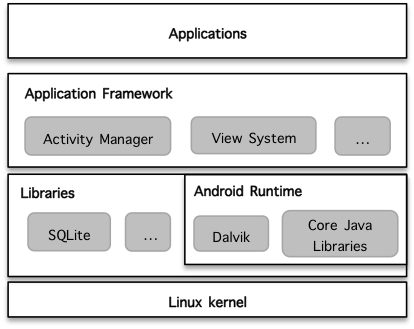
\includegraphics[scale=0.8]{arch3.png}
  \caption{Android Archtecture} \label{fig:exchier} \end{figure}

\subsection{Exception Types in Java} \label{sec:extypes}

In Java, an exception is represented according to the class hierarchy shown in
Figure~\ref{fig:exchier}.  According to it every exception is an
instance of the Throwable class, and can be of three kinds: the checked exceptions
(extends Exception), the runtime exceptions (extends RuntimeException) and errors
(extends Error)~\cite{gosling2000java}. 

The checked exceptions must be specified on the method signature that may throw it, 
and the compiler statically checks if appropriate handlers are provided within the system.
Both runtime exceptions and errors are known as unchecked exceptions, because 
they do not need to be specified on method signatures and do not trigger any 
compile time checking.

By convention an Error represents an unrecoverable condition which usually results
from failures detected by the Java Virtual Machine, such as OutOfMemoryError and
normally should not be handled inside the application. The user-defined exceptions 
can be either checked or runtime. Although the Java specification~\cite{gosling2000java} 
suggests that user-defined exceptions should be checked exception (because doing so 
the callers of a method will know about the exceptions that a method can throw and so 
they can decide what to do about them) there is a long lasting debate about the use of 
checked and unchecked exceptions in Java. 

\begin{figure} \centering 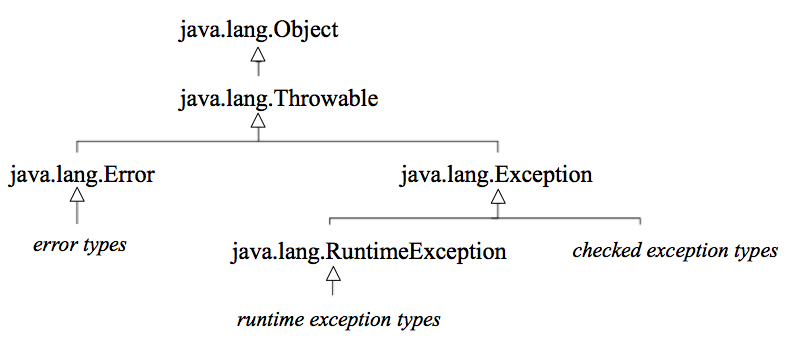
\includegraphics[width=\hsize]{new2_hierarchy.png}
  \caption{Exception Hierarchy in Java} \label{fig:exchier} \end{figure}

The runtime exceptions, however are not only used to represent user-defined
exceptional conditions, they are used by the JVM when a program violates 
the semantic constraints of the Java programming language (out-of-bounds array index, divide-by-zero 
error, null pointer references) from which most of the programs are not expected to recover. 
\footnote{Some programming languages react to such errors by peremptorily terminating the program; 
other programming languages allow similar approaches e.g.C\#; and others let the program to continue
 its execution in some situations such as the out-of-bounds array index e.g., C++. }

%In Java an exception can be thrown in one of the following
%circumstances~\cite{gosling2000java}: 
%(i) explicitly thrown when a throw statement is executed; 
%(ii) implicitly thrown by the JVM when the evaluation of an expression
% violates the normal semantics of language, also refered as a coding error
% (e.g., out-of-bounds array index, division-by-zero, access to a null reference); or 
%(iii) implicitly thrown by the JVM due to an internal error or resource limitation (e.g.,
%OutofMemoryError). 
%\todo{This sub-section is quite similar to the section introduction, shouldn't
%we merge them?}

When an exception is thrown, it causes a transfer of control from the point
where the exception occurred to a point that can be specified by the programmer
(exception handler) - in Java it is represented by the try-catch block . A common way of  
propagating exceptions in Java programs is through exception wrapping
 (also known as exception chaining). Exception wrapping allows one exception 
to be wrapped in another one and re-thrown. Figure~\ref{fig:wrapping} presents 
a stack trace associated which illustrates an exception wrapping. The bottom 
part of the stack trace is the \emph{root cause}, which indicates the
first reason for the error to be thrown (in this case, the computer run out of
memory). The top part of the stack trace indicates the location of the exception
manifestation (which will call \emph{top level exception} along this paper). The
execution flow  between the root cause and the exception manifestation may
include other intermediate exception wrappings. In all levels, the exception
\emph{signaler}, is the method that threw the exception, represented on the
stack trace as the first method call below the exception declaration.

\begin{figure} \centering 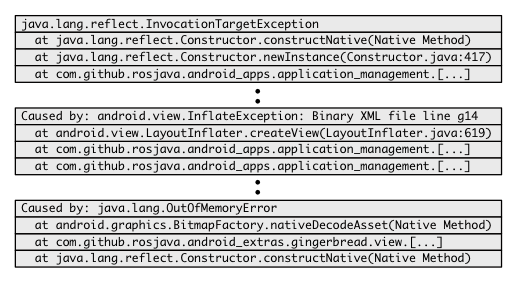
\includegraphics[scale=0.8]{stacktrace.png}
\caption{Example of an Exception stack trace in Java.}
\label{fig:wrapping}
\end{figure}

% \subsection{Public Project Repositories and Issue Trackers} 
% ONE OF THE REVIEWERS COMPLAINED ABOUT THE ABSENCE OF EXPLANATIONS OF WHAT AN ISSU IS...
% As mentioned before, currently more and more projects are becomming available in 
% public project repositories such as GitHub and Google Code.
% Such repositories provides facilities such as....
% The issue trackers available in such projects ....

\subsection{Best Practices}
\label{sec:best}

There is a long-lasting debate about the pros and cons of checked and unchecked exceptions 
~\cite{javatut,stackoverlow,debate},\footnote{152 questions in Stackoverlow
are related to this debate}. Such debates, however, are mainly based on the developers own experience in
using both approaches - since there is a lack of empirical studies on their the pros and cons.

Nevertheless, several general guidelines have been proposed on how to use Java
exceptions~\cite{mandrioli1992advances,gosling2000java,wirfs2006toward,
bloch2008effective} regardless the exception type used. Such guidelines do not focus on 
advocating any specific type but rather propose ways to effectively use each of them.
 We compiled a list of the guidelines related to exception types in Java, 
summarized below:\footnote{We also compiled guidelines related
to exception handling but they are out of the scope of this paper.}

%\noindent\emph{Meaning of Exception Types}

%\textbf{I
\emph{I-Checked exceptions should be used to represent recoverable
conditions} (\cite{mandrioli1992advances,gosling2000java,wirfs2006toward,bloch2008effective})
The developer should use checked exceptions for conditions from which the caller
is expected to recover. By confronting the API user with a checked exception,
the API designer is forcing the client to handle the exceptional condition. The
client can explicitly ignore the exception (swallowing, or converting it to
other type) at the expense of the program's robustness~\cite{gosling2000java}.

\emph{II-Error represents an unrecoverable condition detected by the JVM which
should not he handled} (\cite{gosling2000java}). It results from failures detected
by the Java Virtual Machine which indicate resource deficiencies, invariant
failures or other conditions that make impossible the program to recover.

%\noindent\emph{Exception Throwing}

\emph{III-A method should throw exceptions that precisely define the
exceptional condition} (\cite{gosling2000java,bloch2008effective}). To do so,
developers should either try to reuse the exception types already defined in the
JVM or they should create a specific exception. Throwing general types such as a
pure java.lang.Exception or a java.lang.RuntimeException is considered a bad practice.

%\textbf{IV-Do not repeatedly re-throw exceptions, handle exceptions as close as
%possible to the problem}~\cite{wirfs2006toward}. 
%Programs that frequently throw exceptions lose in performance ~\cite{wirfs2006toward,gosling2000java}.
%Moreover, 
%Close to the place that the exception was throw the caller usually has
%enough contextual information to perform  corrective actions. When the exception
%is propagated far away from the method where it was signaled (i.e. further away
%#from the problem) it can be difficult to take meaningful recovery actions.
%*~\todo{RSC:this practice was not well explored, can be removed if we need space.}

%\noindent\emph{Exception Documentation}
%\textbf{IV- It is wise to document all exceptions thrown by a method} 

\emph{IV- All exceptions explicitly thrown by a method should be documented.}
(\cite{mandrioli1992advances,gosling2000java,wirfs2006toward,bloch2008effective}).
The exceptions thrown by a method are an important part of methods interface,
and is required to use the method properly. The checked exceptions are already
part of the  methods signature, and the method caller is aware of the checked
exceptions being thrown by it. According to~\cite{bloch2008effective}, it is
also wise to document the explicitly thrown runtime exceptions\footnote{This
excludes the implicitly signaled JVM runtime exceptions related to programming
mistakes} as carefully as checked exceptions. Doing so, the clients of a method
will be aware of all the exceptions the method can throw. If the developer fails to
do follow this practice (specially when developing library code) it will be
difficult or even impossible for the caller to make effective use of such 
method~\cite{wirfs2006toward, bloch2008effective} and protect its code
against unforeseen exceptions. 

These best practices guided our exploratory study described next.
Based on information extracted from stack traces (complemented by
bytecode and source-code analysis), we investigate whether stack characteristics
can reveal whether these practices have been obeyed. 
%Next section discusses the
%study procedure and the practices' misuses that emerged from this study.


\section{Empirical Study Design}

The goal of this study was to extract nformation available on exception stack 
traces embedded on issues reported on Android projects, looking for the common characteristics of
those issues and investigating whether they could reveal common defficiencies
on the exception handling code of both the applications and the underlaying 
 framework. 

We choose Android apps because it is the only top platform that is open-source,
and due to its increasing popularity it xxxx.

Our study focused on free apps, since the information needed to perform our study
cannot be retrieved from commercial apps because their issue reports and their
source code is not publicly available. The Android open-source apps were also 
target of other research studies [fse2013][ahimed].   


\subsection{Research Questions}
In the context of our study we formulated the following reseach questions:

\begin{description}

  \item[RQ1] \noindent\emph{What are the common characteristics of exception stack traces reported on issues?} What are the main causes of crashes reported on issues? (more explicit?)

  \item[RQ2] \noindent\emph{What patterns of exception (mis)-use related to exception types and propagation emerge from the exception stack trace analysis?}

\end{description}



%Based mainly on the information available on exception stack traces embedded 
%on issues, the goal of this study was to gain a better understanding 
%of exception-related system crashes.

 
The exceptions available on exception stack traces are not limited to the exceptions 
expliciltly thrown by the Java developer but also include
the exceptions implicitly thrown by the JVM due to programming errors (e.g., out-of-bounds array index, division-by-zero, 
access to a null reference) or resource limitation (e.g., OutOfMemoryError).


For RQ1 and RQ2, we explore the domain quantitatively and highlight interesting cases by 
exploring cases qualitatively. To support this investigation, source code and bytecode 
analysis were used in combination with manual inspection to leverage the  understanding of stack traces and support further discussions and insights. 

\subsection{Data Extraction Process}
\label{sec:miningproc}

The data used in our study to answer our research questions are: the issues related to each 
Android project available in each repository; the source code and manifest file of each application;
the bytecode of all exceptions defined and reused by Android platform.

\subsubsection{Android Apps in GitHub}
\label{sec:git}

As mentioned before, this study amined at mining information available on GitHub issues,
more specifically, extracting and distilling the stack traces embedded on GItHub issues. 
Issues on Github are different from issues on dedicated bug tracking tools such as 
Bugzilla and Jira. The most important difference is that there are no predefined fields
  (e.g. severity and priority). Instead, Github uses a more open ended tagging system, on which
repositories are offered a pre-defined set of labels, but repository owners can modify 
them at will. Therefore, an issue may have none ore an arbitrary set of labels depending 
on which repository it was created. Therefore, this study is based on the assumption 
if an stack trace information embedded in an issue, it contain relevant information
 concerning the exception use -  regardless the lables associated to the issue.

Moreover, issues and pull requests are dual on Github; all pull requests have a corresponding 
``backing'' issue which
are automatically generated. Therefore, we excluded such automatically generated
issues from our analysis. Finally, the Github API allows the automated
generation of issues for specific repositories, which automated tools often use
to report crashes. In some cases, this led to high number of issues that
included stack traces. We identified and filtered those cases out (e.g.,
the~\textsf{pullwifi} project was responsible for almost 50\% of all Android issues in our dataset).

RESUMIR:
This study used the dataset provided by the GHTorrent project~\cite{Gousi13}, an off-line mirror of the data 
offered through the Github API.  GHTorrent has been collecting data from Git since 
February 2012. Up to Dec 2013, and when we queried GHTorrent, it included 332,864 non-fork Java
repositories \footnote {A Java project is specified in GitHub with a
specific label.}  from which only 44,323 have contained at least issue report in their lifetime. From this set only 16,837 were watched by external users. To ensure that our work targets projects that are openly used by
users other than their developers, we focused our analysis on just those projects. 

From this set of 16.836 Java projects which overall contained 356.057 issues, we retrieved the metadata related to each Java project (e.g., repository's names and short descriptions), and the content of every issue and issue comment and stored in a relational database. Using the heuristics presented in Section~\ref{sec:android}, we selected 482 repositories featuring Android projects on which we perform manual inspection was performed.

As mentioned before, in this study we selected a subset of Java projects to
be analyzed in more detail. The subset chosen was comprised by the Android apps
included on GitHub (until 23 Feb 2013).
To identify Android projects, we performed a case insensitive search for the
term \textsf{android} in the repository's names and short descriptions.  The
heuristic filtered 2.542 repositories, from which 589 apps had at least one
issue containing a stack trace.

Then we performed further cleanup, inspecting the site of every Android
reporting at least one stack trace, to make sure that they represented real
mobile apps. During this clean up 106 apps were removed because they were either
example projects (i.e., toy projects) or tools to support Android development
(e.g. \textsf{selendroid}, \textsf{roboeletric} --- tools to support the testing of Android apps).
The filtered set consisted of 482 apps, from which approximately 50\% are also
hosted in Google Market Place. 

This set of 482 projects contained overall 32,582 issues from which 4,208 stacktraces 
were extracted. From this set of issues 44,9\% were labled as defect.


\subsubsection{Android Apps in GoogleCode}

Until January 2014 there were 788 android projects available in Google code repository from which 724 defined at least 1 issue and 183 projects 
had at least one issue including a stack trace. To identify the Android projects on Googlecode we used the search facilities provided looking for 
projects mentioning "Android" on the name of the project or its description. The repository page of each project was inspected, and from this set
142 corresponded to Android applications.

To mine the information available on such Google code projects we implemented a web crawler which navegated on each project and issue page
and extracted the content of each issue to store on relational database. \footnote{Google code previoulsly provided a webservice to extract information about each project, but this service was removed in what Google called "clean-up action" which happened in June 2013.}

\subsection{The ExceptionMiner Tool}
\label{sec:exceptionminer}

To extract exceptions from issues, we implemented ExceptionMiner, a modular
mining tool able to connect to various repositories (such as Google Code,
GHTorrent or even directly to Bugzilla), extract issues, mine stack traces from
them and classify them in predefined categories. The main components of
ExceptionMiner are as follows:

\noindent\emph{Exception StackTrace Miner} The first step in the process is
mining references to exceptions and stack traces embedded in issues, d
GitHub Commector, and GoogleCode Issue Crawler.

\noindent\emph{Exception Stack Trace Distiller} 
Distills the information that composes a stack trace and storing the results in a
relational database. Some of the information extracted from the stack traces were:
 the exception being thrown, its signaler, the exception root cause, its corresponding signaler,
and packages related to each one of these fields.
The tool is based on a combination between a regular expression based parser 
with heuristics able to identify and filter exception names and stack traces inline with text. In
contrast to existing issue parsing solutions such as Infozilla, the parser
created in this work can extract all causes related to an exception on a stack,
and stack traces embedded in logs files.
AS PRESENTED IN FIGURE X

%\begin{tiny}
%\begin{verbatim}

%03-01 W/dalvikvm(7924): threadid=1: thread exiting with uncaught exception (group=0x40adf210)
%03-01 15:55:01.609 (7924): FATAL EXCEPTION: main
%03-01  (7924): java.lang.RuntimeException: ...
%E/AndroidRuntime( 7924):  at android....performLaunchActivity(ActivityThread.java:1967)
%03-01 15:55:01.609 (7924):  at android....handleLaunchActivity(ActivityThread.java:1992)
%03-01 15:55:01.609:  at android.app.ActivityThread.access\$600(ActivityThread.java:127)
%E/AndroidRuntime( 7924):  at android....handleMessage(ActivityThread.java:1158)
%\end{verbatim}
%\end{tiny}

\noindent\emph{Exception Classifier} The next step in the ExceptionMiner process
is classifying exceptions as either checked exceptions, runtime exceptions or 
errors. The exception classifier is based on bytecode analysis (based on Design
Wizard~\cite{Brunet09}) that walks up the type hierarchy of a Java exception
until it reaches a base exception type.

\noindent\emph{Exception Signaler Classifier} After its initialization it
classifies each signaler according to its origin (i.e. Android Plaform,
Aplication, Library, Libcore, or Java) based on pattern matching between the
signaler name and the packages associated to each category.


\subsubsection{The ExceptionMiner Tool}

Before investigating the research questions listed above we analyzed the prevalence of stack traces 
on issues created on Github. Prevalence or prevalence proportion, a term often used in epidemiology,
represents the proportion of a population found to have a particular condition
(e.g. a disease) over the total number of the studied population. In our work, we used
this term to evaluate a condition (i.e., presence of a stack trace) over issues
reported on GitHub repositories.

Using the ExceptionMiner tool, developed in this work, we could extract the exception stack traces defined on issues and issue comments. Executing ExceptionMiner tool each issue and issue comment defined on the 16,836 projects considered in this study, we could observe that 3,758 projects (22,32\%) contained at least 1 issue on which a stack trace was found. Overall the number of issues on which a stack trace was found was 21,013 from which 28,800 stack traces were extracted and analyzed - some issues defined more than one stack trace.

We then analyzed the lables associated to such issues, and we discovered that only 5,196 were labled as defect ~\footnote{the dedect lables considered in this work were every lable containing as substring: defect, bug, crash, failure, fail, exception} (which represent only 24,7\% of the issues on which a stack trace was found), most of the issues on which stack traces were found contained no lable. Such observation supports our assumption to consider not only the issues related with defect issues on this analysis.


\subsubsection{Data Filtering and Manual Inspections}

COMPLETE HERE.....

\subsubsection{Database of Exception Stack Trace Information}
\subsubsection{Distiling Exception Stack Trace Information}

\- root exception
\- signaler
\- method
\- class
\- package
\- Exception

\subsection{Process}

ESPALHAR ESTA SECAO NAS OUTRAS.

Figure~\ref{fig:overviewfig} presents an overview of the mixed-methods approach
conducted to answer these questions. The mixed-methods approach is composed by the following steps:

%\begin{figure*}
%\centering
%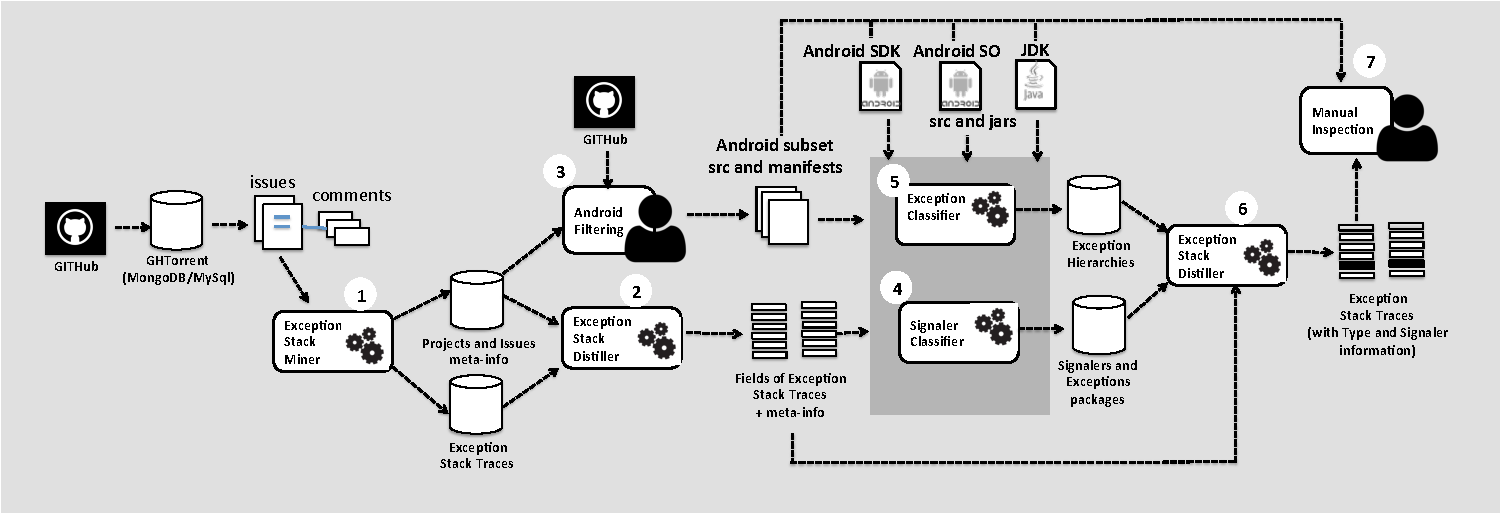
\includegraphics[width=\hsize]{overview.pdf}
%\caption{Overview of the study based on mixed approaches.}
%\label{fig:overviewfig}
%\end{figure*}

%The GHTorrent dataset covers a broad range of
% development activities on Github, including the all the issues per project. Such data 
%is stored in unprocessed format, in a MongoDB database, while metadata is extracted 
%and stored in a relational database. 

\textbf{Step1.} To obtain the Dataset to be analized, we queried GHTorrent as detailed in Section XXX. From GHTorrent we retrieved the metadata related to each Java project (e.g., 
repository's names and short descriptions), and the content of every issue and issue comment 
and stored in a relational database.

\textbf{Step 2.} Extracting Exception Information from Issues. In this step, we used the ExceptionMiner tool,
 developed in this work, to extract the exception names and exception stack traces of each
 issue and issue comment - analyzing the information of each project at a time. This initial 
set of analyzed Java projects included libraries, web-based, Android and stand-alone applications.  

\textbf{Step 3.} Restricting the Dataset to Android Projects. We select a subset of all Android 
projects available on the dataset to perform a deeper analysis (which combined mined
 information extrated from issues with source-code analysis and manual inspection 
of projects resources described on next steps). This decision was driven by the
fact that most open source Anedroid applications are known for dealing
with several sources of exceptions due to multi-threaded execution and
interaction with input/output resources; moreover they share a common
well-defined platform and a limited set of libraries.
To identify Android projects, we performed a case insensitive search for 
the term \textsf{android} in the repository's names and short descriptions.  The
heuristic filtered 2.542 repositories, from which 589 apps had at least one
issue containing a stack trace. Then we performed further cleanup, inspecting the site of every Android
reporting at least one stack trace, to make sure that they represented real
mobile apps. During this clean up 106 apps were removed because they were either
example projects (i.e., toy projects) or tools to support Android development
(e.g. \textsf{selendroid}, \textsf{roboeletric} --- tools to support the testing of Android apps).
The filtered set consisted of 482 apps, from which approximately 50\% are also
hosted in Google Market Place. 

To support a deeper investigation of the stack traces of Android apps, every
exception defined on a stack trace was then classified according to its type
(e.g. Error, Exception or RuntimeException) and to its signaler. To do so, the following 
steps were performed:

\textbf{Step 4.}  Bytecode-Code analysis of JVM and Android Exceptions. We developerd a bytecode analysis tool based on DesignWizard to discover all exceptions thrown by the last version of SDK version 7, and Android Platform and OS (level 19). Every exception was extracted and classified as Runtime, Checked or Error based on the analysis of the exception hierarchy. Our analysis found XXX runtime exceptions in JVM and XX checked, on Android xxx checked and YYY runtime.

\textbf{Step 5.}  Source-Code Analysis of Android Projects. 
For each one of the analyzed projects, we
downloaded the source code and using custom scripts, we extracted their package
hierarchy (recursive list of of Java packages) and their custom exception types.

\textbf{Step 6.}  Manual Inspection. XXXX of the exceptions reported on stack traces  could not be found on JMV, SO or inside the last version of the project. Based on the full name of the exception, a manual inspection was performed on the artifacts associated to the project and libraries used by the project. When even on those sources the exception was not foung [grep-code and similar sites] the exception, in order to discover the exception type. Only 3 exceptions remained undefined and were removed from this study.

\subsection{Replication Package}
All the data used in this study will be publicly available at http://.....
Specifically we provide: (i) all issues related to Android projects found
in GITHub and GoogleCode used in this study; (iii) all stack traces extracted
from issues (ii) the results of manual inspection steps; (iv) the tool developed 
in this work to support stack trace extraction and distilling.

Next section presents the results for each of the study phases, providing both a
quantitative and qualitative analysis of the outcomes.

\section{RQ1: What are the common characteristics of such stack traces?}

%To answer this question, we mined from every extracted stack trace the top level
%exception being signaled, its signaler (the first method signature frame after
%the exception), the root exception (the exception which initiated the stack
%trace, defined on the bottom of the stack), and the root signaler. The
%intermediate elements that compose a stack trace as shown in
%Figure~\ref{fig:wrapping} (i.e., the intermediate causes and its execution
%stacks) were not be considered in the analysis.
%~\todo{Move this to the previous section? IMO, It is better to keep all facts
%about how we did the research in one place
%RSC: I WAS ABOUT TO MOOVE BUT THERE WAS ALREADY A SIMILAR TEXT ON 
%THE EXCEPTION DISTEILLER}

Based on the assumption that regardless the issue type, every exception stack
trace contains relevant information concerning the exception structure of the
projects analyzed, we opted for not restricting the analysis only on defect
issues.\footnote{We conducted the same analysis on the defect issues and the top
exceptions are similar to the ones mentioned on defect issues. Due to space
limitation we limit to present the general analysis here. More detailed analysis
on the defect issues can be found at:
\url{www.dimap.ufrn.br/~roberta/android_repo_mining}}

\subsection{Characterizing the Most Common Root Exceptions}

After distilling the information available on the XXXX  stack traces, extracted from the 
issues and issues comments of XXXX Android projects on GitHub and Googlecode,  
we found XXXX  distinct exceptions reported as the root causes of stack traces.
Table \ref{tab:toptenandroid} illustrates the top 10 root couses found in the study ranked by the number of distinct
project repositories on which they were reported. 

\begin{table*}
  \centering
  \begin{tabular}{rcccccccc}
    \hline
    \bfseries{Root Exception} &  \multicolumn{2}{c}{\bfseries{Projects}} &  \multicolumn{2}{c}{\bfseries{Occurrences}} & \textsf{Android} & \textsf{Libcore} & \textsf{App} & \textsf{Lib} \\
    & \bfseries{\#} &  \bfseries{\%} & \bfseries{\# } & \bfseries{\% } &&&&\\
    \hline
java.lang.NullPointerException            & 254 & 52,70\%  & 1225 & 30,08\% & 473 & 18 & 595 & 137 \\
java.lang.IllegalStateException          & 99  & 20,54\%  & 234  & 5,75\%  & 165 & 12 & 36  & 20  \\
java.lang.IllegalArgumentException          & 94  & 19,50\% & 255  & 6,26\% & 146 & 6  & 64  & 39   \\
java.lang.RuntimeException                & 91  & 18,88\% & 232  & 5,70\%  & 167 & 1  & 47  & 17   \\
java.lang.OutOfMemoryError                 & 56  & 11,62\% & 180  & 4,42\% & 121 & 15 & 17  & 23   \\
java.lang.NoClassDefFoundError           & 52  & 10,79\%  & 73   & 1,79\%  & 9   & 0  & 37  & 26   \\
java.lang.ClassCastException             & 49  & 10,17\%  & 94   & 2,31\%  & 43  & 0  & 40  & 11   \\
java.lang.IndexOutOfBoundsException       & 47  & 9,75\%   & 127  & 3,12\% & 47  & 0  & 71  & 8    \\
java.lang.NoSuchMethodError               & 40  & 8,30\%  & 57   & 1,40\%  & 9   & 0  & 39  & 9   \\
java.util.ConcurrentModificationException & 38  & 7,88\% & 54   & 1,33\%   & 5   & 0  & 43  & 6   \\

    \hline
  \end{tabular}
\caption{Root Exceptions occurrences and popularity.}
\label{tab:toptenandroid}
\end{table*}

%\begin{figure}
%\centering
%\includegraphics[width=\hsize]{top_exceptios_android_new2.pdf}
%\includegraphics[width=\hsize]{top_exceptions_android_new}
%\caption{Top exceptions in Android repositories.}
%\label{fig:androidsignaler}
%\end{figure}

Table \ref{tab:toptenandroid} illustrate the number of times each exception was reported as 
the root cause of a stack trace, the number of distinct projects reporting such causes on stack traces, 
and the percentages of such in relation to all reported exceptions and analyzed projects respectaly.
The table also presents the whether the method responsible for signaling the exceptions were
part of Android, the aplication itself, libcore, or a third-party library as presented in Table  \ref{tab:signalers}  \footnote{9 stack traces contained only elements of JVM and were discarded from the analysis}.

\begin{table}
  \centering
  \begin{tabular}{rp{29em}}
    \hline
    \bfseries{Signaler} & \bfseries{Description} \\
    \hline
    \bfseries{android} & If the exception is thrown by a method defined in Android Platform or OS, or in a JDK library used by them.\\
    \bfseries{app}     & If the exception is thrown by an application method or in a  DK library used by it.\\
    \bfseries{libcore} & If the exception is thrown by one of the core libraries reused by Android (i.e., org.apache.harmony, org.w3c.dom, sun.misc, org.apache.http, org.json, org.xml). \\
    \bfseries{lib}     & If the exception is thrown by a method that was not defined by any of the elements above.\\
    \hline
  \end{tabular}
  \caption{Sources of exceptions in Android}
  \label{tab:signalers}
\end{table}

For each exception we could discover the number of times it occurred on exception stack traces,
the number of distinct projects on which such stacks were defined (and consequently its
popularity) and the of times it was signaled by different signaler types. We
could calculate the popularity of each root cause, considering the number of
distinct projects they were found and the whole set of projects analyzed with at
least one stack trace (482). Table~\ref{tab:toptenandroid} 
%and Figure~\ref{fig:androidsignaler}
presents the mined data.

Programming mistakes are the most common root causes for most types of signalers. We
could observe that the NullPointerException is still the exception with higher
number of occurrences. The NullPoiterExceptions are mainly signaled inside
Android platform and inside application code, although we also find
NullPointerExceptions being signaled from third-party libraries. Regarding
reusable code, there is no consensus whether it is a good or bad practice to 
re-throw
a NullPointerException. Some prefer to encapsulate such an exception on
IllegalArgumentException, while others~\cite{bloch2008effective} argue that the
NullPointerException makes the cause of the problem explicit and hence 
should not be wrapped.

We could observe in this study that the NullPointerException and other
other implicitly signaled exceptions represented most of the exceptions reported
on issues in both Java and Android subset. For such exceptions, which represent
programming bugs or resource limitations, there is usually no proper handling
besides presenting an error message to the user and restarting the application.
Only high fault tolerant systems need to provide solutions to handle them.


----------

We can observe that most of this set is composed by exceptions defined by java.lang,
which are usually implicitly thrown by JMV dur to a programming mistake. From thi set
the java.lang.NullPointerException  was the most reported root cause;  7578 stack traces 
had a java.lang.NullPointerException  as root cause, which corresponds of 26,31\%  of 
all analyzed stack traces. Considering the number of distinct project repositories, 
the java.lang.NullPointerException, was reported on at least one issue of 1,671 projects 
(which represents 44,47\% of all projects reporting at least one stack trace).

The high prevalence of NullPointerExceptions is aligned with the findings other 
works~\cite{kim2013predicting,fraser20131600,csallner2004jcrasher}. For instance, Sunghun et
al.~\cite{kim2013predicting} showed that in Eclipse bug report system 38\% the bugs 
related to exception handling were caused by NullPointerException; other works on robustness 
testing~\cite{maji2012empirical,csallner2004jcrasher} showed that most of the automatically 
detected bugs were due to NullPointerExceptions and implicitly-signaled of Java
environment (as the ones found in this study).

In Section XX we provide further discussion on the NullPointerException problem, pointing 
to ways of how to deal with it and mitigate it.


\subsection{Direct instances of RuntimeExceptions being thrown.}

From Tables~\ref{tab:toptenjava} and~\ref{tab:toptenandroid} we can observe that,
in both Java and Android related issues, direct instances
java.lang.RuntimeException were thrown  in 10,94\% of Java repositories and
18,88\% of Android repositories respectively. 
In the Android repositories, most of such exceptions  were  thrown by the Android 
platform/OS (167 out of 232).

Throwing general exceptions, such as direct instances of RuntimeException, is  considered a
bad practice, because the exception type does not carry enough information to identify the
cause of the exceptional behaviour, and as a consequence developers need to relying on
the exception message which can be neither complete nor precise~\cite{gosling2000java}.





\subsubsection{Classifying Top 100 Exceptions}

To get a broather view of the root causes of stack traces, we performed an empirical evaluation
whose goal was to categorized the top 100 root causes.

After a first inspection of the complete list of exceptions reported, a first set of exception 
categories was defined. This list represent the most common terms reffered on exception
names and javadoc documentation. A similar approach was addopted in [COELHO-ECOOP].
The list of categories is illustrated in Table~\ref{tab:categories}. Hence in the second phase
of the study, each exception was mapped to one of the categories previously defined - 
this analysis was based on the inspection of source code, Javadoc, or additional 
documentation related to the exception. 

To ensure the quality of the classification, three independent coders classified a randomly selected
sample of 25 exception types (from the total 100) using the same categories;
the interater agreement was high (96\%). We can therefore assume that the
categories are descriptive enough for covering the whole range of exception
types that can occur in real world Java projects.


TODO: SEPARAR JAVA DE ANDROID


\begin{table}
  \centering
  \begin{tabular}{|p{2cm}| p{5cm}|}
    \hline
    \bfseries{Category} & \bfseries{Description} \\
    \hline
      Programming logic &  Exceptions thrown by the JVM when the 
evaluation of an expression violates the normal semantics of language (e.g., 
out-of-bounds array index, division-by-zero, access to a null reference). \\ \hline
      Resources (IO, Memory, Energy)  & Exception releated to the manipulation or restriction of resources (e.g., file, network, memory) \\ \hline
      Security                               & Exception releated to security issues (e.g. password validation, criptography) \\ \hline
      Concurrency                            & Exceptions related to multi-threaded programming \\ \hline
      Backward compatibility                 &  A list of exceptions related to backward compatibility - a complete list can be found here [ref]  \\ \hline
      Reflection                             & Exceptions related to Java reflection library  \\ \hline
      Specific                & Exceptions created for specific applications, frameworks or libraries \\ \hline
      General (Exception, Error, Runtime)    & The top level exceptions in Java    \\ \hline
    \hline
  \end{tabular}
  \caption{Description of categories.}
  \label{tab:categories}
\end{table}

The top 100 root causes correspond to approximately 77\% of all stack traces
reported reported on Java stack-issues and 95\% of all exceptions reported on
Android stack-issues. Table~\ref{tab:tophundrend} illustrates the result of such 
classification.

\begin{table}
  \centering
  \begin{tabular}{lrr}
    \hline
    \bfseries{Category} &  \bfseries{ Ocurrences (\%)} \\
    \hline
      Programming logic (java.lang and util) & 2235 (55,64\%)\\
      Resources (IO)                         &  727 (18,10\%) \\
      Security                               &  165 (4,11\%)\\
      Concurrency                            & 116  (2,89\%)\\
      Backward compatibility                 &  219 (5,45\%) \\
      Reflection                             &  91 (2,27\%)\\
      Specific (GUI,FRAMEWORK)               &  197 (4,90\%)\\
      General (Error, Exception, Runtime)    &  267 (6,65\%)\\
    \hline
  \end{tabular}
  \caption{Characterization of the 100 root causes.}
  \label{tab:tophundrend}
\end{table}

Programming errors are the causes of most of the exception stack traces reported
on issues both in  general Java data set and Android subset. In the Android subset we could find 
more stack traces reporting exceptions related to Backward
compatibility and security concerns than on the general data set.


TODO: Discuss about the interater agreement here...

%\subsection{Sizes of Stack traces}
%Concerning the size of the stacks (i.e. the number of frames composing them), we
%could observe that  sometimes it exceeded 100 frames (158 stack frames).
%Manually inspecting the corresponding execution trace was caused by one of the
%two reasons: recursive calls or exceptions signaled by a method defined deep
%down in a reused framework; exceptions successively wrapped. Irrespective of the
%reason, in exception flows involving many methods, it is practically impossible
%to handle an exception in a way other than exiting the application, as at the
%place the exception occurs there is hardly enough contextual information to
%perform recovery actions.

%Considering only the packages of each exception we could observe that 81,28\%
%of all analyzed set of stack traces reported exceptions defined by java.lang
%(see Table XXX).

%\begin{table}
% \centering
%\begin{tabular}{lrrrr}
%    \hline
% \bfseries{rank} & \bfseries{package} & \bfseries{occurr} &  \bfseries{\%occur} & % \bfseries{projects} \\
%     \hline
%1 & java.lang         & 19471 & 81,28\% & 3080 \\
%2 & java.io           & 1222  & 5,10\%  & 509 \\
%3 & java.net          & 740   & 3,09\%  & 311 \\
%4 & java.util         & 689   & 2,88\%  & 287 \\
%5 & java.lang.reflect & 115   & 0,48\%  & 78 \\
%\hline
%  \end{tabular}
%\caption{Top 5 most popular packages associated to the root exceptions of stack traces}
%\label{tab:toptenpopular2}
%\end{table}

%\noindent \fbox{
%\begin{minipage}{0.96\columnwidth} 
%\emph{RQ2: Most exceptions are due to programming mistakes
%or generally irrecoverable errors.}
%\end{minipage}}

\section{RQ2.  What kinds of exception (mis)-use emerge from stack trace analysis? }

To answer this question we: (i) distilled the information available on stack traces (i.e., exception signalers, root causes, exception wrappings); 
(ii) mined the exception types related to each exception reported on stack traces using source code and byte code analyses; and finally checked 
this information against the compiled best practices. Doing so, we mined some characteristics of exception stack traces that points to best practices violations.

 Table~\ref{tab:typeroottab} presents the types of root causes of all stack traces reported on the analyzed issues. As we can see 
from Table ~\ref{tab:typeroottab},  most of the reported exceptions were signaled by Android and libraries reused by Apps were runtime exceptions. 
On the other hand, we could observe that most of the reported exceptions signaled by the set of 
libraries reused by Android platform (i.e., org.apache.harmony,
org.w3c.dom, sun.misc, org.apache.http, org.json, org.xml, javax -- referred in
this work as libcore) were checked exceptions. It is pointed as a good practice
for libraries (see Section~\ref{sec:best}) because by using checked exceptions
libraries can define a precise exception interface to its clients. Such
libraries are heavily used in several projects, and such precise exception
interface may be related to the library's maturity.


\begin{table}
\centering
\begin{tabular}{lccccc}
    \hline
    \bfseries{Root Cause Type} & \bfseries{Android} & \bfseries{Libcore} & \bfseries{App} & \bfseries{Lib}  & \bfseries{All}\\
    \hline

Runtime	&	1075	&	56	&	1446	&	374	&	2951\\
Error	&	144	&	34	&	168	&	105	&		451	\\
Checked	&	110	&	230	&	139	&	145	&	624	\\
Throwable	&	0	&	0	&	1	&	0	&	1	\\
Undefined	&	1	&	0	&	6	&	8	&	15	\\
    \hline
All		& 1330	&	320	&	1760	&	632	&	4042	\\
    \hline
  \end{tabular}
\caption{Types of root exceptions.}
  \label{tab:typeroottab}
\end{table}


%\begin{figure}
%\centering
%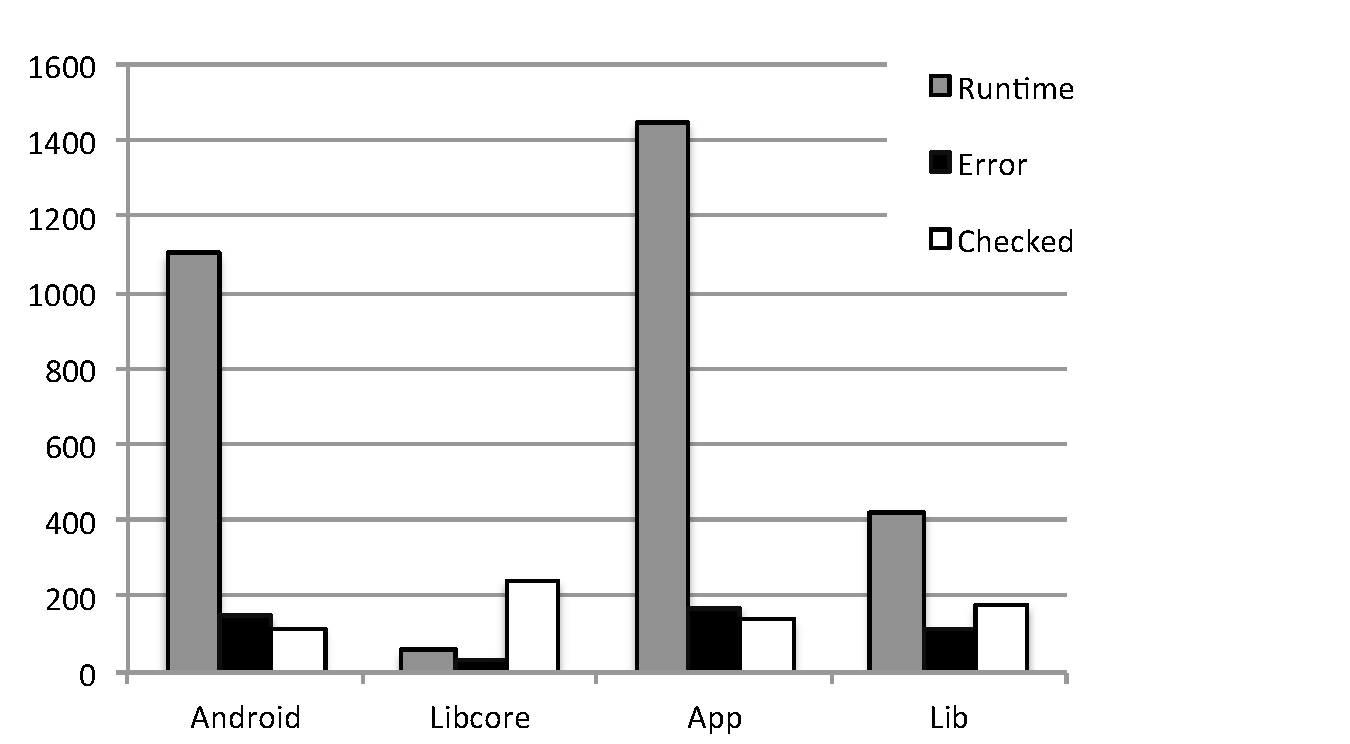
\includegraphics[width=\hsize]{chart_exceptiontypes.pdf}
%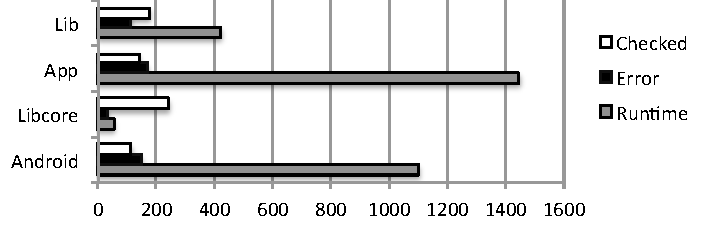
\includegraphics[width=\hsize]{exception_types.pdf}
%\caption{Distribution of Checked and Unchedked exceptions.}
%\label{fig:typeroot}
%\end{figure}


% REMOVED BECAUSE WE DO NOT HAVE SPACE TO DISCUSS IT, AND IT IS NOT WELL
% CONNECTED WITH PREVIOUS.
%\subsection{Uncaught Checked Exceptions}
%Although most of the  reported exceptions were runtime, we could also find checked
%exceptions as the root causes of stack traces reported on issues. A checked exception
%can remain uncaught in two circumstances: if all methods on the execution trace
%on which this exception flows explicitly specifies the exception, or if the
%checked exception is wrapped in a runtime and than re-thrown. Since checked exceptions 
%should be used to represent recoverable conditions, ignoring a
%checked exception, is considered a bad practice. As mentioned before, when the developer is confronted
%with a checked exception, the designer of the API is telling him to handle the
%exceptional condition. To better understand what was causing checked exceptions
%to scape from being handled we investigated the kinds of wrappings that happened
%on stacks the stacks.  Next sections presents the wrappings found and discuss
%about them.


\subsection{What can the Exception Wrappings tell us?}

Table~\ref{tab:wrappingandroid} presents the wrappings found in this study for all
stack traces found in Android repositories. As we can see, some of the checked
exceptions were indeed wrapped in runtime exceptions or even errors, while most
of them were not wrapped along the stack trace. 



\begin{table*}
  \centering
  \begin{tabular}{llcccccc}
    \hline
    \bfseries{Wrapper Type}  &  \bfseries{Root Cause Type} &  \bfseries{Projects}  &  \bfseries{Occurrences} & \textsf{Android} & \textsf{Java/Libcore} & \textsf{Lib} & \textsf{App}  \\
    \hline
      Runtime &  Checked   & 70 & 114 & 66 &  0  & 19 &  29 \\
      Runtime   &  Error   & 38  & 57 & 50 &  0  & 6 &  1 \\
      Checked &  Runtime   & 12 & 22 & 4 &  0  & 9 &  9 \\
      Checked & Error      & 7 &  8 & 5 &  0  & 0 &  3 \\
      Error & Checked      & 4  &  7 &  &  0  & 7 &  0     \\
      Error & Runtime     & 6  &  13   & 1 &  1  & 0 &  11    \\
    \hline
  \end{tabular}
\caption{Wrappings comprising different exception types.}
\label{tab:wrappingandroid}
\end{table*}

This analysis also revealed unexpected wrappings such as: Error wrapping a Checked 
exception; a Runtime wrapping and Error; and an Error wrapping a Runtime.
Java is the only language that provides a hybrid exception handling mechanism
which offers  different types to represent different exception behaviors (i.e., error, 
runtime and checked) (see Section~\ref{sec:best}). According to Java specification Errors should not be
handled inside the system since they usually represent unrecoverable conditions
detected by the JVM such as OutOfMemoryError. Checked exceptions should
represent recoverable conditions and  Runtime exceptions represent are usually
related to programming mistakes from which the developer is not expected to recover
from. 

\subsubsection{Runtime wrapping Checked Exception}

Such wrapping was detected on distinct 70 projects. Inspecting the 
elements responsible for performing such wrapping we could observe that,
most of such wrappings were perform on methods defined on Android. 


\begin{table}
\centering
\begin{tabular}{ll}
    \hline
    \bfseries{signaler from} & \bfseries{Ocurrences} \\
    \hline
ANDROID	 & 66 \\
APP	& 29 	(HOW MANY?? AND WHICH??) \\
LIB  & 19 (HOW MANY AND WHICH?)\\
\hline
  \end{tabular}
\caption{Elements responsible for the wrapping.}
\label{tab:wrapping01}
\end{table}


Taking a closer look on the signalers reposponsible for wrapping we could observe that, aproximately 41%
of all wrappings were performed by a single class, called ActivityThread, responsible for managing the life cycle 
of an Android application. It performs the application callbacks.


\begin{table}
\centering
\begin{tabular}{ll}
 \bfseries{Signaler class} & \bfseries{Ocurrences} \\
    \hline
android.app.ActivityThread & 47 \\
android.view.LayoutInflater & 7 \\
org.gege.caldavsyncadapter.syncadapter.SyncAdapter & 7 \\
org.springframework.web.client.RestTemplate & 6 \\
android.os.AsyncTask & 5 \\
\hline
  \end{tabular}
\caption{Elements tresponsible for the wrapping.}
\label{tab:wrapping01}
\end{table}

Code snipet extracted from android.app.ActivityThread.

{\footnotesize
\begin{verbatim}

private Activity performLaunchActivity(...) {
  try {
   ...
  } catch (Exception e) {
    ...
    throw new RuntimeException(..., e);
  }
}
\end{verbatim}
}

The exceptions most wrapped on RuntimeExceptinos were:


\begin{table}
\centering
\begin{tabular}{lll}
    \hline
    \bfseries{wrapper} & \bfseries{root} & \bfseries{\#} \\
    \hline
java.lang.RuntimeException & java.lang.ClassNotFoundException &	32 \\
java.lang.RuntimeException & java.lang.NoSuchMethodException &	6 \\
java.lang.RuntimeException & java.lang.InstantiationException) & 5 \\
...andlyticsproject.NetworkException & org.apache...HttpResponseException &	5\\
android.view.InflateException & java.lang.NoSuchMethodException & 4 \\
\hline
  \end{tabular}
\caption{Elements tresponsible for the wrapping.}
\label{tab:wrapping01}
\end{table}


\begin{table}
\centering
\begin{tabular}{lll}
    \hline
    \bfseries{Exception} & \bfseries{Ocurrences} \\
    \hline
java.lang.RuntimeException &	69 & 61\% \\
android.view.InflateException	& 10 & 8,7\% \\
com.github.andlyticsproject.console.NetworkException	& 7 & - \\
java.lang.IllegalStateException	& 6 & - \\

\hline
  \end{tabular}
\caption{Elements tresponsible for the wrapping.}
\label{tab:wrapping01}
\end{table}



\subsubsection{Runtime Exception wrapping Error}


 We could find  57 stack traces on 38 projects on which an Error was wrapped in a Runtime Exception.



\begin{table}
\centering
\begin{tabular}{ll}
 \bfseries{Signaler from} & \bfseries{Ocurrences} \\
    \hline
ANDROID	& 50 \\
LIB  & 6 \\
APP	& 1 \\
\hline
  \end{tabular}
\caption{Elements tresponsible for the wrapping.}
\label{tab:wrapping01}
\end{table}


\begin{table}
\centering
\begin{tabular}{ll}
 \bfseries{Signaler method} & \bfseries{Ocurrences} \\
    \hline
android.os.AsyncTask &	25 \\
android.app.ActivityThread & 15 \\
android.view.LayoutInflater & 7 \\
org.asynctasktex.AsyncTaskExd & 3 \\
android.support.v4.content.ModernAsyncTask & 2\\
\hline
  \end{tabular}
\caption{Elements tresponsible for the wrapping.}
\label{tab:wrapping01}
\end{table}


EXAMPLE: android.os.AsyncTask

{\footnotesize
\begin{verbatim}
protected void done() {
 ...
   try {
      ...
   } catch (InterruptedException e) {
      android.util.Log.w(..., e);
   } catch (ExecutionException e) {
      throw new RuntimeException("...",e.getCause());
   } catch (CancellationException e) {
      ...
   } catch (Throwable t) {
     throw new RuntimeException("...", t);
   }
    ...
 }
}
\end{verbatim}
}

%SELECT (exception, root_cause) AS PAIR, COUNT (*) AS N FROM stacktracesummary where 
%EXCEPTION_EXTENDS='RUNTIME' AND ROOT_EXTENDS='ERROR' GROUP BY PAIR ORDER BY N DESC;



\begin{table}
\centering
\begin{tabular}{ll}
 \bfseries{Signaler method} & \bfseries{Ocurrences} \\
    \hline
java.lang.RuntimeException,java.lang.OutOfMemoryError & 30\\
java.lang.RuntimeException,java.lang.NoClassDefFoundError & 6\\
java.lang.RuntimeException,java.lang.UnsatisfiedLinkError) & 5\\
android.view.InflateException,java.lang.OutOfMemoryError) & 4\\
java.lang.RuntimeException,java.lang.StackOverflowError)  & 4\\
\hline
  \end{tabular}
\caption{Elements tresponsible for the wrapping.}
\label{tab:wrapping01}
\end{table}

TO INVESTIGATE: WHICH WERE THE LIBS AND THE APP? AND ITS REPUTATION?

\subsubsection{Checked wrapping Runtime Exception}



\begin{table}
\centering
\begin{tabular}{ll}
 \bfseries{Origin} & \bfseries{Ocurrences} \\
    \hline
APP	& 9 \\
LIB	& 9 \\
ANDROID &	4 \\
\hline
  \end{tabular}
\caption{Elements tresponsible for the wrapping.}
\label{tab:wrapping01}
\end{table}
\begin{table}
\centering
\begin{tabular}{lll}
 \bfseries{Wrapper} & \bfseries{Root} & \bfseries{Ocurrences}\\
 \hline
...android.robospice.CacheSavingException,java.lang.ClassCastException & 6 \\
java.lang.reflect.InvocationTargetException,java.lang.NullPointerException &  3 \\
java.lang.reflect.InvocationTargetException,android...ResourcesdNotFoundException & 2 \\
java.sql.SQLException,android.database.sqlite.SQLiteDiskIOException & 2 \\
java.lang.Exception,at.andiwand.odf2html.odf.IllegalMimeTypeException & 	2 \\
  \end{tabular}
\caption{Elements tresponsible for the wrapping.}
\label{tab:wrapping01}
\end{table}


The most frequent exception wrapping were were performed inside RoboSpice is an android library that supports the creation of asynchronous long running tasks.
This library has 1.682 stars and 367 forks.

Most of such wrappings however were caused by the reflection Java library, used by Android, Application and library classes.
relaction methods convert every exception thata happens when invoking a reflected method into an INVOCATION TARGET EXCEPTION
this conversion is performed inside native code.

\subsubsection{Checked Exception wrapping Error}

We could observe that in 7 projects this  wrapping happend 8 times in total.
Inspecting the stack traces we could observe that 7 out of 8 wrappings were caused
by the reflection java library on which java.lang.OutOfMemoryError
java.lang.NoSuchMethodError were wrapped into a java.lang.reflect.InvocationTargetException.

\begin{table}
\centering
\begin{tabular}{ll}
 \bfseries{Origin} & \bfseries{Ocurrences} \\
    \hline
ANDROID	& 5 \\
APP	& 3 \\
  \end{tabular}
\caption{Elements tresponsible for the wrapping.}
\label{tab:wrapping01}
\end{table}


\begin{table}
\centering
\begin{tabular}{lll}
 \bfseries{Wrapper} & \bfseries{Root} & \bfseries{Ocurrences}\\
 \hline
java.lang.reflect.InvocationTargetException,java.lang.OutOfMemoryError & 5 \\
java.lang.Exception,java.lang.OutOfMemoryError & 1 \\
java.lang.reflect.InvocationTargetException,java.lang.NoSuchMethodError &	1 \\
java.lang.reflect.InvocationTargetException,java.lang.UnsatisfiedLinkError&	1 \\
  \end{tabular}
\caption{Elements tresponsible for the wrapping.}
\label{tab:wrapping01}
\end{table}

All wrappings except 1 were caused by the reflection library.
The method responsible for the wrappings (e.g., at java.lang.reflect.Constructor.constructNative(Native Method))
were native methods written in C. In one of the cases, however, in project OpenDocument.droid a java.lang.Exception was 
wrapping a java.lang.OutOfMemoryError. General handlers are considered as bad practice, 
but wrapping an Error on a general Exception make the matters worse.

\subsubsection{Error wrapping Checked Exception}

%SELECT (exception, root_cause) AS PAIR, COUNT (*) AS N FROM stacktracesummary where 
%EXCEPTION_EXTENDS='ERROR' AND ROOT_EXTENDS='CHECKED' GROUP BY PAIR ORDER BY N DESC;


\begin{table}
\centering
\begin{tabular}{ll}
libcore	&  3 \\
 JAVA ENV  & 	4 \\
  \end{tabular}
\caption{Elements tresponsible for the wrapping.}
\label{tab:wrapping01}
\end{table}



\begin{table}
\centering
\begin{tabular}{lll}
 \bfseries{Wrapper} & \bfseries{Root} & \bfseries{Ocurrences}\\
 \hline
java.lang.NoClassDefFoundError & java.lang.ClassNotFoundException & 4 \\
java.lang.AssertionError & javax.crypto.ShortBufferException) & 3 \\
 \end{tabular}
\caption{Elements tresponsible for the wrapping.}
\label{tab:wrapping01}
\end{table}

Some wrappings were performed by methods defined by java.lang.Class methods such as 
at java.lang.Class.getDeclaredFields(Native Method)
at java.lang.Class.getDeclaredConstructors(Native Method).  While were performed by javax.crypto package.

\subsubsection{Error wrapping Runtime}

\begin{table}
\centering
\begin{tabular}{ll}
APP & 11 \\
ANDROID	& 1 \\
LIB	& 1 \\
  \end{tabular}
\caption{Elements tresponsible for the wrapping.}
\label{tab:wrapping01}
\end{table}


\begin{table}
\centering
\begin{tabular}{lll}
 \bfseries{Wrapper} & \bfseries{Root} & \bfseries{Ocurrences}\\
 \hline
java.lang.ExceptionInInitializerError,java.lang.NullPointerException & 9 \\
java.lang.ExceptionInInitializerError,java.lang.IllegalArgumentException &	2 \\
java.lang.ExceptionInInitializerError,java.util.MissingResourceException) &	1 \\
java.lang.ExceptionInInitializerError,org.andengine.util.exception.AndEngineRuntimeException &	1 \\
 \end{tabular}
\caption{Elements tresponsible for the wrapping.}
\label{tab:wrapping01}
\end{table}

after manually inspecting the code associated to such wrappings we discovered that all of them were 
caused by static initializers. If any exception is thrown in the context of a static initializer (i.e., static block) 
it is converted into an ExceptionInitializerError on the point where the class is first used.

%Table X illustrated examples of such wrappings.
%TODO INCLUIR ESTA TABLEA

%\begin{figure}
%  \begin{center}
%    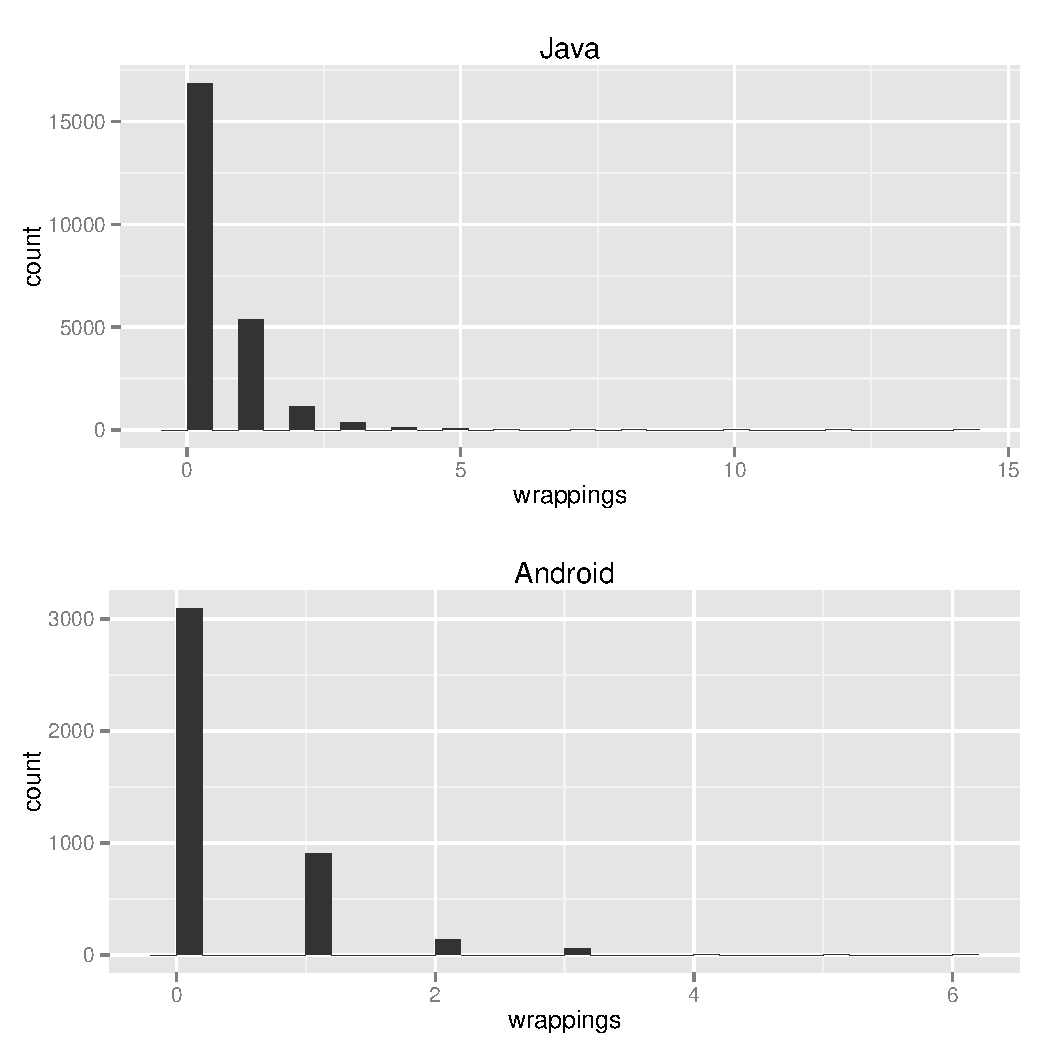
\includegraphics[scale=0.4]{stack-wrappings-hist.pdf}
%  \end{center}
%  \caption{Number of stack traces wrappings for Java and Android repositories. }
%  \label{fig:sizewrapbhists}
%\end{figure}


\subsubsection{Multiple Wrappings}

We could also observe that in 205 stacks found in Android repository the exception was wrapped 
more then once. Figure ~\ref{fig:sizewrapbhists}  illustrates the number of wrappings per stack, both
 in Java and Android studied repositories. One interesting multiple-wrapping found in Android repo was the 
following: Runtime-Checked-Runtime-Checked-Runtime-Checked-Runtime.

\subsection{What can the Signalers tell us?}

After investigating the most popular exceptions on issues, we also investigated elements
responsible for signaling most of the exceptions reported on issues.
Such elements were directly involved on the reported crashes. We cannot
directly blame such component for the crash since the client may not have been
using the component according to its "contract", or an external event
may have happened during the execution of such method.

Regardless the reason, such analysis give as a clue to comon element involved on 
reported crashes. Table X illustrates the most common root exception signalers
on issues, toglether with the list of exceptions being thrown.

%Present the top signalers found in this study, and top pairs (signalers and exceptions), and discuss 
%about inversion of control and the difficult to adequately handle exceptions in this style of development.
%Inversion of control stimulate the use of unchecked exceptions since the "call back" do not know which exception to expect.

{\tiny
\begin{verbatim}

% SELECT mainsignaler_method,count(distinct(repo)) as n, string_agg(distinct(main_cause), ',')
% FROM stacktracesummary group by (mainsignaler_method) order by n desc;

GITHUB:
"android.os.Parcel.readException";28;"Exception,java.lang.IllegalArgumentException,java.lang.IllegalStateException,java.lang.NullPointerException,java.lang.SecurityException"
"dalvik.system.BaseDexClassLoader.findClass";19;"java.lang.ClassNotFoundException"
---> "android.app.Instrumentation.checkStartActivityResult";17;"android.content.ActivityNotFoundException"
"android.graphics.BitmapFactory.nativeDecodeStream";16;"java.lang.OutOfMemoryError"
--->"android.view.WindowManagerImpl.findViewLocked";15;"java.lang.IllegalArgumentException"
"android.graphics.Bitmap.nativeCreate";15;"java.lang.IllegalArgumentException,java.lang.OutOfMemoryError"
"android.graphics.BitmapFactory.nativeDecodeAsset";14;"java.lang.OutOfMemoryError,java.lang.RuntimeException"
"dalvik.system.PathClassLoader.findClass";13;"java.lang.ClassNotFoundException"
---> "android.support.v4.app.FragmentManagerImpl.checkStateLoss";12;"java.lang.IllegalStateException"
"android.os.BinderProxy.transact";12;"android.os.DeadObjectException,android.os.TransactionTooLargeException,java.lang.RuntimeException"
"android.database.DatabaseUtils.readExceptionFromParcel";11;"android.database.sqlite.SQLiteDiskIOException,android.database.sqlite.SQLiteException,java.lang.IllegalArgumentException"
"android.app.ActivityThread.performLaunchActivity";11;"java.lang.NullPointerException,java.lang.RuntimeException"
--->"android.graphics.Canvas.throwIfRecycled";10;"java.lang.NullPointerException,java.lang.RuntimeException" (private method throwing a RuntimeException)
--->"android.os.StrictModedAndroidBlockGuardPolicy.onNetwork";10;"android.os.NetworkOnMainThreadException" (public)
---> "android.support.v4.app.Fragment.getResources";10;"java.lang.IllegalStateException"
"android.os.AsyncTaskd3.done";10;"java.lang.RuntimeException"

"The Canvas class holds the "draw" calls. To draw something, you need 4 basic components: A Bitmap to hold the pixels, a Canvas to host the draw calls (writing into the bitmap), a drawing primitive (e.g. Rect, Path, text, Bitmap), and a paint (to describe the colors and styles for the drawing)."

"private static void More ...throwIfRecycled(Bitmap bitmap) {
941         if (bitmap.isRecycled()) {
942             throw new RuntimeException(
943                         "Canvas: trying to use a recycled bitmap " + bitmap);
944         }
945     }"


GOOGLECODE:
"android.app.Instrumentation.checkStartActivityResult";8;"android.content.ActivityNotFoundException"
"android.graphics.Bitmap.nativeCreate";8;"java.lang.IllegalArgumentException,java.lang.OutOfMemoryError,java.lang.RuntimeException"
"java.lang.ClassLoader.loadClass";6;"java.lang.ClassNotFoundException,java.lang.IncompatibleClassChangeError,java.lang.UnsupportedClassVersionError"
"dalvik.system.BaseDexClassLoader.findClass";6;"ClassNotFoundException,java.lang.ClassNotFoundException"
"com.android.dx.dex.file.ClassDefsSection.add";6;"java.lang.IllegalArgumentException"
"android.os.Parcel.readException";6;"Exception,java.lang.IllegalArgumentException,java.lang.IllegalStateException,java.lang.NullPointerException,java.lang.SecurityException"
"android.view.WindowManagerImpl.findViewLocked";5;"java.lang.IllegalArgumentException"
"android.os.BinderProxy.transact";5;"android.os.DeadObjectException,android.os.RemoteException,android.os.TransactionTooLargeException,java.lang.RuntimeException,java.lang.SecurityException"
"android.app.ActivityThread.performLaunchActivity";5;"Error,java.lang.NullPointerException,java.lang.RuntimeException"
"android.graphics.BitmapFactory.nativeDecodeStream";5;"java.lang.OutOfMemoryError"


\end{verbatim}
}

\subsection{Undocumented runtime exceptions.} After filtering out all the exceptions implicitly 
signaled by  JVM (due to programming mistakes) and inspecting the signaler methods of such exceptions (i.e.,  direct an indirect 
instances of java.lang.RuntimeException). We could observe that only 1 method out of 118 inspected signalers
 (i.e., 0,8\%) documented the explicitly thrown runtime exception in a Javadoc comment; and none of these methods
included the runtime exception  (reported on the stack) as part of the exception interface of the method (i.e., using 
throws clause on method signature). This result is aligned with the results of other  study conducted by from 
Sacramento et al ~\cite{sacramento2006unchecked} which observed that the
runtime exceptions in .Net programs are most often not documented.

Such undocumented runtime exceptions represent a threat to system robustness, specially
when such exceptions are thrown then the third party code is invoked inside the application (e.g. libraries, or framework utility code).
In such cases the client usually do not have access to the source code, and in the absence of
the exception documentation it is very difficult or even impossible for the client of such third party code to 
protect the application against undocumented runtime exceptions. As a consequence, the
 undocumented runtime exception may remain uncaught and lead to system crashes.


\section{Discussions and Actionable Advices}

The exception (mis-)use patterns that emerged  in this study sheds light on 
problems that may be reducing the robustness of current Java programs in the face of
exceptional conditions. 

Discuss about the actionable advices propagated by TAO XIE.


%\noindent\emph{The undocumented runtime exceptions} 
\subsection{The undocumented runtime exceptions thrown by thrid party code} 
Documenting runtime exceptions is a tedious and error prone task, to help developers
mitigate this problem tools should be developed to automate the documentation of runtime exceptions
scraping from library code, few solutions in this directions have been proposed so far ~\cite{van2005combining}. 

%\noindent\emph{The odd wrappings}  
\subsection{Exception Wrappings: Language design purpose x real use}

The exception wrappings were inicially proposed by Java [ref-specification] to ...

But the types of wrappings found in this study pointing to the fact that some wrappings may have not 
been used according to its intial purpose. It can sometimes be used to bypass the  
language restrictions imposed by checked exceptions.

When (mis)applied, the exception wrapping can lead to what we call
an \emph{exception handling confusion problem} which can lead the program to
an unpredictable state in the presence of exceptions. To illustrate this problem, we can use
 one of the examples found in this study: when the developer is 
confronted with a checked exception, the designer of the API is telling him 
to handle the exceptional condition, however we could observe that in some cases the 
checked exception wrapped an OutOfMemoryError, which represent resource deficiency detected 
by the JVM which make impossible the program to recover. Further investigation is needed on finding 
ways to help developers in deadling with such problem, either preventing odd wrappings or enabling 
the developer to better deal with them. 


\subsubsection{Ways of Preventing Odd Wrappings}
Since there is no way of enforcing Java exception type conventions during program development,
the exceptions regardless its types can se used interchangeably. This interchangeability makes the
behaviour of the exception handling code more complex and less reliable. For
instance, considering a situation were an instance of OutOfMemoryError (a situation that usually cannot
 be handled) was wrapped in a checked exception which tells the caller that such exception should
handled.


\subsection{Checked and Unchecked Exceptions in JVM and Android and what they can tell us?}

We could observe that some of the type-changing-wrappings were performed by JDK classes.
Such finding lead us to think that the exception types have been used as intercheagable and may not being carrying 
the meaning they were firstly designed to carry.

The way the exceptions are being handle are more important that the type itself, it points to the fact already discussed 
by other languages such as M\# blog [ref] and \"thinking in Java author\" and other blogs. It is all about the exception handling
politics of a system and not the type itself. The exception type is not enought to ensure a more strict or robust development,
since the checked exceptions may be silienced or converted to a checked exception. According to Java manual,
they say that it can actually happen but it will be done intentionally and they advocate that it is a bad practice.

Present the number of checke and unchecked exceptions in JVM, JDK, Android SO, and Android SDK.
Discuss about the amount of checked and unchecked defined in each, and discuss about interesting exceptions that
have the same name ex: classNotFound...



%\noindent\emph{The high number of null pointer exceptions}  

\subsection{The high number of null pointer exceptions}  

The null references was firstly introdduced by Tony Hoare in ALGOL W, which after some years he called his “one-billion-dollar mistake”:

"I call it my billion-dollar mistake. It was the invention of the null reference in 1965 [...] I couldn’t resist the temptation to put 
in a null reference, simply because it was so easy to implement. This has led to innumerable errors, vulnerabilities, and system 
crashes, which have probably caused a billion dollars of pain and damage in the last forty year."

ref: http://bertrandmeyer.com/category/computer-science/

The high number of null pointer exceptions found in this mining study shed light into a problem
that although known was not supported by large scale mining studies on the large.  

This observation emphasises the importance of solutions to avoid NullPointerExceptions, such as:
(i) lightweight intra-method nullpointer analysis supported by Java8 @Nullable annotations;
(ii) intermethod nullpointer analysis tools such as the one proposed by [DANIELE-RELATED-WORK];
or (iii) whether language designs which avoid null pointers, such 
as Monads ~\cite{Walde95} (i.e., used in functional languages for values that may not be available 
or computations that may fail) could improve the robustness of Java programs. 

The @Nullable annotations are used by analyzers like the Checker Framework, FindBugs, Eclipse, 
NetBeans, IntelliJ, and other commercial tools which run at compile time and detect potential null 
pointer derecefences. Android Studio 0.5.5 Released support these annotations.


(1) mostrar a utilizacao de @nullable em projetos android. rodar em alguns e mostrar.
Android Project Unwritten Rules (http://blog.lemberg.co.uk/android-project-unwritten-rules)

(2) dar foco em android

(3) falar do modelo do ciclo de vida da aplicacao e da necessidade de usar excecoes Runtime.

(4) Local onde tratar excecao - handler padrao - politica da aplicacao. tratamento difucultado multiplas threads e assyncronos.




%\noindent\emph{Dependency injection - Inversion of Control -  callback and Exceptions }  
\subsection{Dependency injection - Inversion of Control -  callback and Exceptions}  

%\noindent\emph{How can we benefit from such cross-project crash analysis?}  
\subsection{The benefits of a cross-project crash analysis}  

When family of systems make use of a common core, or framework such systems can
bennefit from a cross project crash analysis. The bug issues reported for a group of systems
can identify vulnerabilities which were more difficult to identify in a single project analysis.

The test case explosion problem... A test suite is always incomplete,
one application could benefit from the usage scenarios on which such framework is applied.
Framework testing -  what are the main challenges wor framework testing?
A crossproject crash analysis based on repository mining techniques can 
identify vulnerabilitues in pieces of code that are shared. 

Using exception miner tool we could identify the methods reponsible for most of the crashes - 
such methods can be a target for manual inspections improvements, or better documentation
(because sometimes an exception can be thrown because the user is not invoking the method
in the proper way 

During such analysis we could also find the undocumented runtime exceptions 
signaled by libraries. 

It allows the developers to benefit from the faults happening on different systems.


\subsection{Actionable Advices - The Unwrittern rules of Android development}


%The results of a mining study should be a set of actionalble advices (tao xie).


\section{Threats to Validity}

\noindent\emph{Internal Validity} We used a heuristics-based parser to mine
exceptions from issues.  Our parsing strategy was conservative by default; for
example, we only considered exception names using a fully qualified class name
as valid exception identifiers, while, in many cases, developers use the
exception name in issue description. Conservative parsing may minimize false
positives, which was our initial target, but also tends to increase false
negatives, which means that some cases may have not been identified as
exceptions or stack traces. Our limited manual inspection did not reveal such
cases.

\noindent\emph{External Validity} The results presented here were based on mining
issues on Github through the GHTorrent dataset. While comprehensive and
extensive, GHTorrent is not an exact replica of Github, so several issues might
be left out. Due to the way data collection works with GHTorrent, for projects
that are relatively inactive, GHTorrent might have not collected a significant
proportion of their issues. We did not investigate the extend of this threat on
our sample.

\noindent\emph{Construct Validity} Parts of our analysis are based on the availability of stack traces on issues on
Github. In using this dataset, we make an underlying assumption: the
stack traces reported on issues are representative of real crashes in
the applications. The assumption is impossible to mitigate without access to
the full set of crash data per application. Services exist to collect all
crash data from applications, so access to such a dataset will allow for
a thorough replication of our analysis, perhaps at the individual application
level.

\section{Related Work}

In this section, we present work that is related to the present paper, divided into
three categories: i) papers that use the information available on stack traces;
ii) empirical studies on the usage of Java exceptions and its fault proneness;
and iii) tools to extract stack traces information from natural language artifacts
(e.g., issues and emails).
%, and iv) empirical studies involving Android apps.


\textit{Empirical studies using Android apps.} Ruiz et al.~\cite{Ruiz12}
investigated the degree of reuse across applications in Android Market, the
study showed that almost 23\% of the classes inherited from a base class in the
Android API, and that 217 mobile apps were reused completely by another mobile
app. Pathak et al.~\cite{Patha11} analyzed bug reports and developers
discussions of Android platform and found out that approximately 20\% of
energy-related bugs in Android occurred after an OS update. McDonnell et
al.~\cite{McDon13} conducted a case study of the co-evolution behavior of
Android API and 10 dependent applications using the version history data found
in github. The study found that approximately 25\% of all methods in the client
code used the Android API, and that the methods reusing fast-evolving APIs were
more defect prone then others. Vásquez et al.~\cite{Linar13} analyzed
approximately 7K free Android apps and observed that the last successful apps
used Android APIs that were on average 300\% more change-prone than the APIs
used by the most successful apps. Pingyu and Elbaum~\cite{Zhang12} analyzed bug
reports of 5 Android applications an observed that 29\% had to do with poor
exceptional handling code. Our work differs from the others as it aims at
distilling the information of bug reports describing uncaught exceptions created
for mobile applications in Github, in order to get a first view
of what is causing the crashes across applications available and what the
characteristics of the stack traces can tell us about the exception structure of
those applications.

\textit{Extracting Stack Traces from natural language artifacts.} 
%Currently, many
%software vendors embed automatic crash reporting tools in their software
%systems. Moreover, third party crash collection services exist, most of them 
%targeted for applications run on mobile phones~\cite{BugSe14,BugSn14,Googl14,Acra14}.
Apart from bug reports, stack traces can be embedded in other forms of
communication between developers, such as discussion logs and emails.
Being intermixed with text makes the accurate extraction of stacktraces 
an involved process.
Infozilla~\cite{bettenburg2008extracting}
is based on a set of regular expressions that extract a set of frames
related to a stack trace. The main limitation of this solution is that it is not
able to extract stack traces embedded on verbose log files (i.e., on which we
can find log text mixed with exception frames). Bacchelli
et al.~\cite{bacchelli2012content} propose a solution to recognize stack trace frames
from development emails and relate it to code artifacts (i.e. classes) mentioned
on the stack trace. In addition to those tools, ExceptionMiner is able to 
both extract stack traces from natural language artifacts and to 
classify them in a set of predefined categories.
(MENCIONAR QUE X% DOAS EXCECOES ANALISADAS ESTAVAM EMBEBIDAS EM ALGUM TIPO DE ARQUIVO DE LOG - 
LOGCAT DO ANDROID....)


\textit{Analysis and Use of Stack Trace Information.} Several works have
investigated the use of stack trace information to support bug classification
and clustering~\cite{wang2013improving, kim2011crash, dhaliwal2011classifying},
fault-proneness prediction models~\cite{kim2013predicting} and even automated
bug fixing tools~\cite{sinha2009fault}. Kim et al.~\cite{kim2011crash} use an
aggregated form of multiple stack traces available in crash reports to detect
duplicate crash reports and to predict if a given crash will be fixed. Dhaliwal
et al.~\cite{dhaliwal2011classifying} proposed a crash grouping approach that
can reduce bug fixing time in approximately 5\%. Wang et
al.~\cite{wang2013improving} propose an approach to identify correlated crash
types and describe a fault localization method to locate and rank files related
to the bug described on a stack trace. Schroter et al.~\cite{schroter2010stack}
conducted an empirical study on the usefulness of stack traces for bug fixing
and showed that developers fixed the bugs faster when failing stack traces were
included on bug issues.  In a similar study, Bettenburg et
al.~\cite{bettenburg2008makes} identify stack traces as the second most stack
trace feature for developers.  Sinha et al.~\cite{sinha2009fault} proposed an
approach that uses stack traces to guide a dataflow analysis for locating and
repairing faults that are caused by the JVM implicitly signaled exceptions. Kim
at al.~\cite{kim2013predicting} proposed an approach to predict the
crash-proneness of methods based information extracted from stack traces and
methods' bytecode operations.  They observed that most of the stack traces were
related to NullPointerException and other JMV implicitly thrown exceptions had
the higher prevalence on the analyzed set of stacks.


\textit{Tools Support for Detecting Faults on Java Exception Handling Code.} 

Manually analyzing the exception handling code looking for defects, can easily 
become infeasible [ref]. Hence, some tools have been proposed to detect faults 
on the exception handling code either statically (cabral, roberta,nelio,chang) 
or dynamicaly through testing (roberta). Both approaches, however, have inherent
 limitations. On the one hand, the static analysis tools needs to deal with the false 
positives and cannot adequately deal with dynamically loaded code (e.g. reflection  
[ref]). On the other hand the testing tools are llimited to the fact that the developer
 needs to create a test to exercise every exception, which is also costly.... (olhar tese). 
Moreover, both methods fail to account for exceptions implicitly signaled by the runtime 
environment (e.g. due to resource depletion which can be signaled in every statement invocation). 

Robillard and Murphy~\cite{Robil00}
employed dataflow analysis to find the propagation paths of checked and
unchecked exception types. Modeled after Robillard and Murphy's work, other
tools have been proposed to support the static analysis of exception
flows~\cite{coelho2008assessing}. The main limitation of all
static analysis tools is the number of false positives inherent to static analysis
solutions, which can lead to a high number of exception flows, specially if
considering Java Environment exceptions and exceptions signaled from libraries.
 
Additionally, Cabral and Marques~\cite{cabral2007exception} analyzed the
exception handling code of 32 open-source systems, both for Java and .NET. They
observed that the action handlers were very simple (e.g., logging and present a
message to the user). Reimer and Srinivasan~\cite{reimer2003analyzing} listed a
set of bad practices on exception handling that hinder software maintainability
and robustness, based on their own experience with Java enterprise applications.
Our work differs from those two works as we tried to identify bad practices from
the analysis of stack traces extracted from issues in combination with and bytecode and source
code analysis. 


\enlargethispage{-2\baselineskip}

\section{Conclusion}

In this paper we present an exploratory study in which we mined the stack 
traces embedded in all issues of Java projects available GitHub.
Furthermore, we analyzed in more detail the
stack traces reported on a subset of 482 Android projects. In this study, the information extracted 
from stack traces was used in combination with source code and bytecode analysis to 
pin-point patterns of exception use and misuse in Java.
Certain patterns of exception
(mis)-use were consistently detected such as unexpected wrappings (e.g., Errors
being wrapped in checked exceptions), revealing that  the Java hybrid exception
model is not fully used according to its purpose; undocumented runtime
exceptions signaled by third party code (which makes it almost impossible for
library clients to protect against such exceptions); 
and a high prevalence of
\texttt{java.lang} exceptions reported on issues (representing approximately 50\% of the
analyzed issues). Such (mis)uses detected in our study can negatively affect the 
robustness of current Java software systems. Our results call for  
 developing tools support to help developers dealing with such problems and 
improving the design of the exception handling mechanism in Java.

%Nowadays many software vendors embed automatic crash reporting tools in their
%software systems. Hence, whenever a software crashes this tool sends a detailed
%crash report to its vendors. Moreover, we can also find third party sofware
%solutions specialized in bug reporting for different kinds of systems specially
%for the increasing marked of mobile apps~\cite{BugSe14,BugSn14,Googl14,Acra14}.
%There is planty of information to be mined...





\begin{table}
\centering
\begin{tabular}{llll}
    \hline
    \bfseries{Project} & \bfseries{merging imeStars} & \bfseries{Watchers} & \bfseries{Forks} \\
    \hline
subsampling-scale-image-view  &  -  &  -    & - \\
Android-PullToRefresh &  -  &  -    & - \\
HackerNews &  -  &  -    & - \\
PathfinderOpenReference  &  -  &  -    & - \\
AndroidStaggeredGrid  &  -  &  -    & - \\
HtmlSpanner  &  -  &  -    & - \\
screen-notifications  &  -  &  -    & - \\
appdatapreferences-android  &  -  &  -    & - \\
Android-Universal-Image-Loader  &  -  &  -    & - \\
Android-SDK  &  -  &  -    & - \\
WebCachedImageView  &  -  &  -    & - \\
Android-SkyDrive-Browser  &  -  &  -    & - \\
android-pdfview  &  -  &  -    & - \\
hn-android  &  -  &  -    & - \\
Android-BitmapCache  &  -  &  -    & - \\
cropper  &  -  &  -    & - \\
WordPress-Android  &  -  &  -    & - \\
changeloglib  &  -  &  -    & - \\
cgeo  &  -  &  -    & - \\
chromium-webview-UNDERLINE  &  -  &  -    & - \\
AndroidSlidingUpPanel  &  -  &  -    & - \\
DsaTab  &  -  &  -    & - \\
box-android-sdk-v2  &  -  &  -    & - \\
chromeview  &  -  &  -    & - \\
andlytics  &  -  &  -    & - \\
ContractionTimer  &  -  &  -    & - \\
android  &  -  &  -    & - \\
okhttp  &  -  &  -    & - \\
ActionBarSherlock  &  -  &  -    & - \\
mobile-android  &  -  &  -    & - \\
android-timepicker  &  -  &  -    & - \\
QuiltViewLibrary  &  -  &  -    & - \\
congress-android  &  -  &  -    & - \\
c-geo-opensource  &  -  &  -    & - \\
TweetLanes  &  -  &  -    & - \\
PageTurner  &  -  &  -    & - \\
SWADroid  &  -  &  -    & - \\
picasso  &  -  &  -    & - \\
uservoice-android-sdk  &  -  &  -    & - \\
\hline
  \end{tabular}
\caption{Projects containing wrappings Error-Runtime}
\label{tab:wrappings3}
\end{table}

The methods performing such wrappings were the following:

%source code of ActivityThread -  https://github.com/android/platform_frameworks_base/blob/master/core/java/android/app/ActivityThread.java

\begin{table}
\begin{tabular}{l}
    \hline
    \bfseries{root signaler -  occurences} \\
      \hline
android.app.ActivityThread.handleBindApplication – 2 \\
android.app.ActivityThread.performLaunchActivity – 13 \\
android.os.AsyncTaskd3.done – 25	 \\
android.support.v4.content.ModernAsyncTaskd3.done - 2 \\
android.view.LayoutInflater.createView - 7 \\
android.view.Viewd1.onClick - 1 \\
com.squareup.picasso.Requestd1.run - 1 \\
me.openphoto.android.app.util.concurrent.AsyncTaskExd3.done - 1 \\
org.asynctasktex.AsyncTaskExd3.done – 3 \\
org.chromium.androidwebview.AwBrowserProcess.loadLibrary -1 \\
org.gradle.groovy.scripts.internal.DefaultScriptRunnerFactorydScriptRunnerImpl.run - 1 \\
\hline
  \end{tabular}
\caption{Top 10 most popular exceptions on issues in Java projects}
\label{tab:toptenjava}
\end{table}







\subsection{Exception Handling in Programming Languages}

Techniques for error detection and handling are not  an optional add-on but a
fundamental part of any system~\cite{bruntink2006discovering}. 
The exception mechanism~\cite{goodenough1975exception} was proposed as a way of
preventing errors from being ignored and was embedded in many mainstream
programming languages ~\cite{garcia2001comparative} since then. 

In languages such as Modula-3, Guide, and Extended Ada the exceptions are 
checked, which means that the compiler statically checks if appropriate handlers 
are provided within the system. Accordingly, the programmer must explicitly specify 
every exception that can be signaled to support the compile time checking. This approach is known to be
costly to maintain (Dooren and Steegmans, 2005) since exception updates are
cascading; if a new exception type is added to a method signature then all other
methods directly using this method must either change their signatures to
include the new exception type or handle the new exception. 

In languages such as Lore, C++, and Arche all exceptions are unchecked but the developer can 
optionally list exception types on method signatures. Although exceptions can 
be documented on methods signatures, the developer is not warned by the compiler
if an unchecked exception is not handled inside the application. According to ~\cite{Robil00} 
such an approach may hinder robustness because the client of a method cannot easily know
which unchecked exceptions may be thrown (unless the code of the method and the
methods called from it is inspected) which can be a very time consuming or
infeasible task. 

Java [ref: Gosling et al. 1996] and CLU [Liskov and Snyder 1979] support the checked exceptions,
 (therefore the compiler can then check if handlers are provided to such exceptions), however, this support is 
only partial because both languages also provides a form of unchecked exceptions [ref: Robilard].
In CLU,  if a handler is not found for a given exception, it is automaticaly converted in a predened default exception, 
called failure which is the only one which can be implicitly propagated [ref-clue].
 In Java the developer can define specific unchecked and checked exceptions and use both kinds in a single system.

There is a long-lasting debate about the pros and cons of checked and unchecked exceptions 
~\cite{javatut,stackoverlow,debate},\footnote{152 questions in Stackoverlow
are related to this debate}. However, the debates are mainly based on the developers own experience in
using both models, since there is still few empirical evidence of the pros and cons of each model.

%Although exception handling mechanism has been embedded in several programming languages 
%as show above,  the exception handling code is often poorly understood and the least
%tested part of software systems [ref:POORLY]. 

%[REF]: Static Analysis to Support the Evolution of Exception Structure in Object-Oriented Systems

% This behaviour may lead to the problem of uncaught exceptions~\cite{jo2004uncaught}, one of the main causes of application crashes
%(e.g.~\cite{miller1997issues,Robil00,shah2010understanding, garcia2007extracting, garcia2001comparative,cabral2007exception,coelho2011unveiling}).






\section*{Acknowledgment} This work is partially supported by: CNPq -- Proc.
484209/2013-2 and the NWO TestRoots project (639.022.314).


\bibliographystyle{IEEEtran}
\bibliography{android-stacks}

% that's all folks
\end{document}

